% Created 2019-09-09 Пн 00:07
% Intended LaTeX compiler: pdflatex
\documentclass[11pt]{article}
\usepackage[utf8]{inputenc}
\usepackage[T1]{fontenc}
\usepackage{graphicx}
\usepackage{grffile}
\usepackage{longtable}
\usepackage{wrapfig}
\usepackage{rotating}
\usepackage[normalem]{ulem}
\usepackage{indentfirst}
\usepackage{amsmath}
\usepackage{textcomp}
\usepackage{paracol}
\usepackage{amssymb}
\usepackage{capt-of}
\usepackage{hyperref}
\usepackage[T2A]{fontenc}
\usepackage[a4paper,left=3cm,top=2cm,right=1.5cm,bottom=2cm,marginparsep=7pt,marginparwidth=.6in]{geometry}
\usepackage{cmap}
\usepackage[russian, english]{babel}
\usepackage{xcolor}
\usepackage{listings}
\author{АВТОР}
\date{\today}
\title{}
\hypersetup{
 pdfauthor={АВТОР},
 pdftitle={},
 pdfkeywords={},
 pdfsubject={},
 pdfcreator={Emacs 26.1 (Org mode 9.1.9)}, 
 pdflang={Rusian, English}}
\begin{document}

\large
\thispagestyle{empty}
\begin{center}
\textbf{Санкт-Петербургский Национальный Исследовательский}\\
\textbf{Университет Информационных Технологий, Механики и Оптики}\\
\textbf{Факультет Программной Инженерии и Компьютерной Техники}\\
\end{center}
\vspace{1em}
\begin{center}

\includegraphics[width=120px]{../../itmo-logo.png}
\end{center}
\LARGE
\vspace{5em}
\begin{center}
\textbf{Вариант № 30}\\
\textbf{Лабораторная работа № 1}\\
\Large
\textbf{по дисциплине}\\
\LARGE
\textbf{\emph{'Информатика'}}\\
\end{center}
\vspace{11em}
\large
\begin{flushright}
\textbf{Выполнил:}\\
\textbf{Студент группы P3113}\\
\textbf{\emph{Куперштейн Дмитрий;} : 269359}\\
\textbf{Преподаватель:}\\
\textbf{\emph{МАЛЫШЕВА ТАТЬЯНА АЛЕКСЕЕВНА}}\\
\end{flushright}
\vspace{4em}
\large
\begin{center}
\textbf{Санкт-Петербург 2019 г.}
\end{center}
\pagebreak{}
\setcounter{tocdepth}{2}
\renewcommand{\contentsname}{Оглавление}
\tableofcontents
\pagebreak{}
\section{Задание}
\begin{enumerate}
    \item Перевести число "А", заданное в системе счисления "В", в систему
счисления "С". Числа "А", "В" и "С" взять из представленных ниже
таблиц. Вариант выбирается как сумма последнего числа в номере
группы и номера в списке группы согласно ISU. Т.е. 13-му человеку
из группы P3102 соответствует 15-й вариант (=2 + 13).
    \item Всего нужно решить 11 примеров. Для примеров с 5-го по 7-й
выполнить операцию перевода по сокращенному правилу (для систем
с основанием 2 в системы с основанием $2^k$). Для примеров с 4-го по
6-й и с 8-го по 9-й найти ответ с точностью до 5 знака после запятой.
В примере 11 группа символов \{\^{}1\} означает -1 в симметричной
системе счисления.
\end{enumerate}
Далее числа A, B и С привидены в начале заданий согласно таблице для варианта 30\\
\pagebreak{}
\section{Решение}
\small
\begin{paracol}{2}
\noindent
\begin{enumerate}
    \item$A = 99518\quad B = 10\quad C = 11$
    \\\\
    $95518_{10} = 65845_{11}$
    \\\\
    $
    \arraycolsep=0.05em
    \begin{array}{rrrrr@{\,}r|rrrr@{\,}r|rrr@{\,}r|rr@{\,}r|r@{\,}r}
    9&5&5&1&8 &&\, 1&1\\
    \cline{7-10}
    8&8 &&&&& 8&6&8&3 &&\, 1&1\\
    \cline{1-3} \cline{12-15}
    & 7&5 && &&\, 7&7&& &&\, 7&8&9 &&\, 1&1\\
    \cline{7-9} \cline{15-19}
    & 6&6 && &&\, &9&8& &&\, 7&7& &&\, 7&1 &&\, 1&1\\
    \cline{2-4} \cline{12-13} \cline{18-20}
    & &9&1& &&\,&8&8 && &&\,1&9 &&\, 6&6 &&\, \textbf{6}\\
    \cline{8-10} \cline{16-18}
    & &8&8& &&\, &1&0&3 &&\, &1&1 &&\, \textbf{5}\\
    \cline{3-5} \cline{13-15}
    &&&3&8 &&\, &&9&9 &&\, &&\textbf{8}\\
    \cline{8-10}
    &&&3&3 &&\, &&&\textbf{4}\\
    \cline{4-5}
    &&&&\textbf{5}\\
    \end{array}
    $
    \item$A = 89373\quad B = 11\quad C = 10$
    \\\\
    $89373_{11} = 129550_{10}$
    \\\\
    $89373_{11} = 3 \cdot 11^0 + 7 \cdot 11^1 + 3 \cdot 11^2 + 9 \cdot 11^3 + 8 \cdot 11^4 = 129550$
    \item$A = 2E6ED\quad B = 15\quad C = 15$
    \\\\
    $2E6ED_{15} = 14300243_{5}$
    \\\\
    $2E6ED_{16} = 13 \cdot 15^0 + 14 \cdot 15^1 + 6 \cdot 15^2 + 14 \cdot 15^3 + 2 \cdot 15^4 = 150073$
    \\\\
    %$
    %\arraycolsep=0.05em
    %\begin{array}{rrrrrr@{\,}r|rrrrr@{\,}r|rrrr@{\,}r|rrrr@{\,}r|rrr@{\,}r|rr@{\,}r%|r@{\,}r|r@{\,}r}
    %1&5&0&0&7&3 &&\,5\\
    %\cline{7-13}
    %1&5&0&0&7&0 &&\, 3&0&0&1&4 &&\, 5\\
    %\cline{1-6} \cline{13-17}
    %&&&&&\textbf{3} &&\, 3&0&0&1&0 &&\, 6&0&0&2 &&\, 5\\
    %\cline{7-12}\cline{18-22}
    %&&&&&& &&\, &&&\textbf{4} && 6&0&0&0 &&\, 1&2&0&0 &&\, 5\\
    %\cline{13-17} \cline{23-27}
    %&&&&&& &&\, &&& &&\, &&&\textbf{2} &&\, 1&2&0&0 &&\, 2&4&0 &&\, 5\\
    %\cline{18-22} \cline{28-30}
    %&&&&&& &&\, &&& &&\, &&&& &&\, &&\textbf{0} &&\, 2&4&0 &&\, 4&8 &&\, 5\\
    %\cline{23-27} \cline{30-31}
    %&&&&&& &&\, &&& &&\, &&&& &&\, && &&\, &&\textbf{0} &&\, 4&5 &&\, 9 &&\, 5\\
    %\cline{28-30} \cline{33-33}
    %&&&&&& &&\, &&& &&\, &&&& &&\, && &&\, && &&\, &\textbf{3} &&\, 5 &&\, %\textbf{1}\\
    %\cline{30-31}
    %&&&&&& &&\, &&& &&\, &&&& &&\, && &&\, && &&\, & &&\, \textbf{4} &&\, \\
    %\end{array}
    %$
    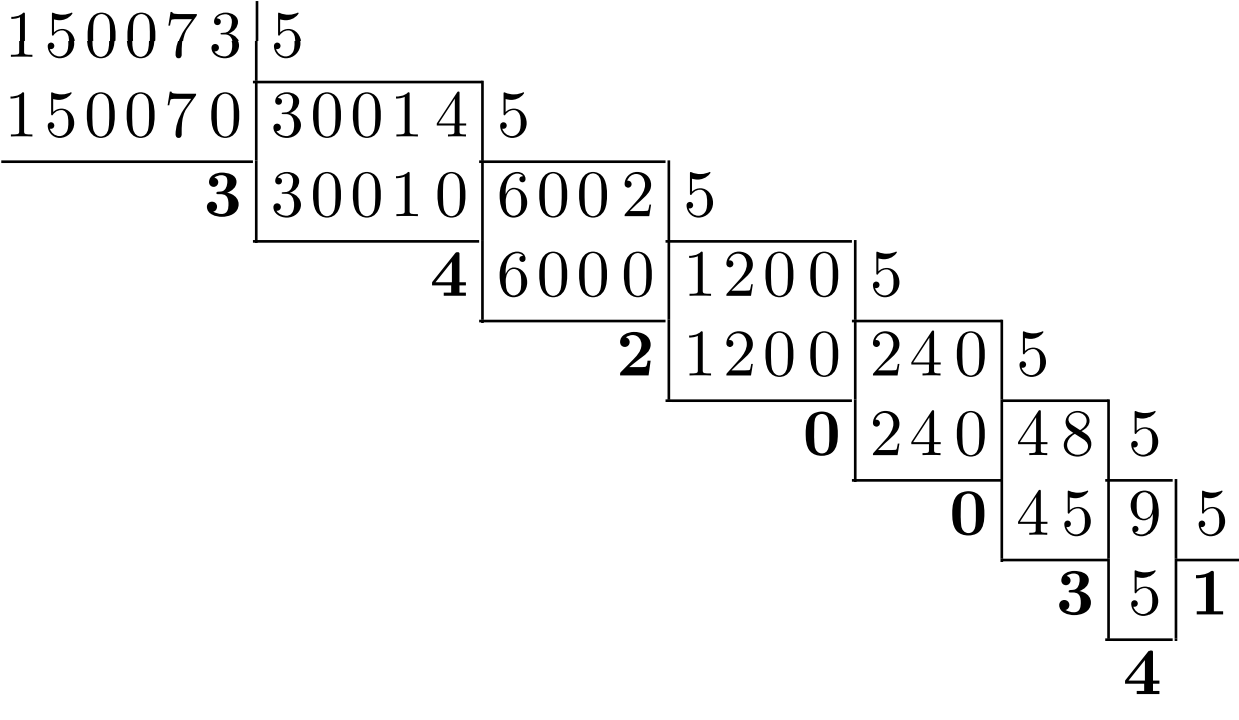
\includegraphics[width=156px]{3.png}
    \item$A = 68,41\quad B = 10\quad C = 2$
    \\\\
    $68,41_{10} \approx 1000100,01101_{2}$
    \\\\
    Методом подбора переводим целую часть (68)
    в двоичную систему: $68 = 2^6 + 2^2$, т.е.
    \\\\
    $68_{10} = 1000100_{2}$
    \\\\
    Отдельно переведём дробную часть (0,41)
    с точностью до пяти знаков
    \\\\
    $0,41 \cdot 2 = 0,82 \quad 0$\\
    $0,82 \cdot 2 = 1,64 \quad 1$\\
    $0,64 \cdot 2 = 1,28 \quad 1$\\
    $0,28 \cdot 2 = 0,56 \quad 0$\\
    $0,56 \cdot 2 = 0,12 \quad 1$\\
    \item$A = B5,12\quad B = 16\quad C = 2$
    \\\\
    $B5,12_{16} \approx 10110101,00010_2$
    \\\\
    \switchcolumn
    Переводим отдельно целую часть и дробную
    (с точностью до пяти знаков)
    тетрадами с отбросом незначущих нулей
    \\\\
    \begin{tabular}{|c|c|c|c|@{}l}
    \cline{1-4}
    B & 5, & 1 & 2 & $\,_{16}$\\
    \cline{1-4}
    1011 & 0101, & 0001 & 0100 & $\,_2$\\
    \cline{1-4}
    \end{tabular}
    \setcounter{enumi}{5}
    \item$A = 25,22\quad B = 8\quad C = 2$
    \\\\
    $25,22_8 = 10101,01001$
    \\\\
    Переводим отдельно целую часть и дробную
    (с точностью до пяти знаков)
    триадами с отбросом незначущих нулей
    \\\\
    \begin{tabular}{|c|c|c|c|@{}l}
    \cline{1-4}
    2 & 5, & 2 & 2 & $\,_8$\\
    \cline{1-4}
    010 & 101, & 010 & 010 & $\,_2$\\
    \cline{1-4}
    \end{tabular}
    \item$A = 0,101001\quad B = 2\quad C = 16$
    \\\\
    $0,101001_{2} = 0,A4_{16}$
    \\\\
    Целая часть равно нулю, переводим дробную
    тетрадами, отделяя тетрады,
    считая от запятой:
    \\\\
    \begin{tabular}{c|c|c|@{}l}
    \cline{2-3}
    0, & 1010 & 0100 & $\,_2$\\
    \cline{2-3}
    0, & A & 4 & $\,_{16}$\\
    \cline{2-3}
    \end{tabular}
    \item$A = 0,101101\quad B = 2\quad C = 10$
    \\\\
    $0,101101_2 \approx 0,70313_{10}$
    \\\\
    $0,101101_{2} = 2^{-1} + 2^{-3} + 2^{-4} + 2^{-6} = 0,703125$
    \\\\
    Округляем до пятого знака после запятой
    \item$A = 28,D2\quad B = 16\quad C = 10$
    \\\\
    $28,D2_{16} \approx 40,82031_{10}$
    \\\\
    Переводим отдельно целую и дробную часть
    \\\\
    $28_{16} = 8 \cdot 16^0 + 2 \cdot 16^1 = 40$
    \\\\
    $0,D2_{16} = 13 \cdot 16^{-1} + 2 \cdot 16^{-2} = 0.8203125$
    \item$A = 105\quad B = 10\quad C = \text{Фиб}$
    \\\\
    $105 = 1000100100_{\text{Фиб}}$
    \\\\
    Определяем, что 89 максимальное число\\ Фибоначчи, меньшее 105, остальные\\ слагаемые определяем подбором:
    \\\\
    $105 = 89 + 13 + 3 = 1000100100_{\text{Фиб}}$
    \item$A = 2\{\string^1\}33\{\string^3\}\quad B = 7C\quad C = 10$
    \\\\
    $2\{\string^1\}33\{\string^3\}_{7C} =4624$
    \\\\
    $2\{\string^1\}33\{\string^3\}_{7C} = -3 \cdot 7^0 + 3 \cdot 7^1
    + 3 \cdot 7^2 + -1 \cdot 7^3 + 2 \cdot 7^4 = 4624$
    \\\\
    
\end{enumerate}
\end{paracol}
\section{Таблица ответов}
\large
\begin{tabular}{|c|c|}
\hline
№ & Ответ\\
\hline
1 & 65845\\
\hline
2 & 129550\\
\hline
3 & 14300243\\
\hline
4 & 1000100,01101\\
\hline
5 & 10110101,00010\\
\hline
6 & 10101,01001\\
\hline
7 & 0,А4\\
\hline
8 & 0,70313\\
\hline
9 & 40,82031\\
\hline
10 & 1000100100\\
\hline
11 & 4624\\
\hline
\end{tabular}
\\\\
\section{Вывод}
В ходе этой лабораторной работы я закрепил навыки работы с разными системами счисления и различными алгоритмами
для перевода чисел из одной СС в другую, а так же укрепил теоретические знания и познакомился с СС на базе чисел Фибоначчи.
\end{document}
